\documentclass[../../main.tex]{subfiles}

\graphicspath{{../../fig/}}
\setcounter{section}{0}

\begin{document}

\chapter{宇宙マイクロ波背景放射(CMB)}
宇宙マイクロ波背景放射(Cosmic Microwave Background: CMB)とは、宇宙の創生から38万年後に物質から脱結合した光子のことであり、我々が観測できる最古の光である。
その発見はペンジアスとウィルソンによって1965年に行われ\cite{1965ApJ...142..419P}、
その後Cosmic Background Explorer(COBE)衛星により強度の周波数依存性(スペクトル)が測定された\cite{1996ApJ...473..576F}。
測定されたスペクトルは温度が$\SI{2.725}{K}$の黒体輻射のスペクトルと一致し(図\ref{fig:cobe})、CMBがほとんど一様等方な強度を持つことも確認された。
これらの事実によりCMBはビッグバン宇宙モデルを支持する強力な証拠となった。
こうして現代の宇宙論の基礎を築き、発展させてきたCMBは、現在ではその偏光情報からインフレーション宇宙論の証拠を探ることができると期待されている。
本章では、はじめに現在の標準的な宇宙モデルである$\Lambda\mathrm{CDM}$モデルについて述べ、次いでインフレーション宇宙論について述べる。
その後、CMB偏光について述べる。
\begin{figure}[H]
    \centering
    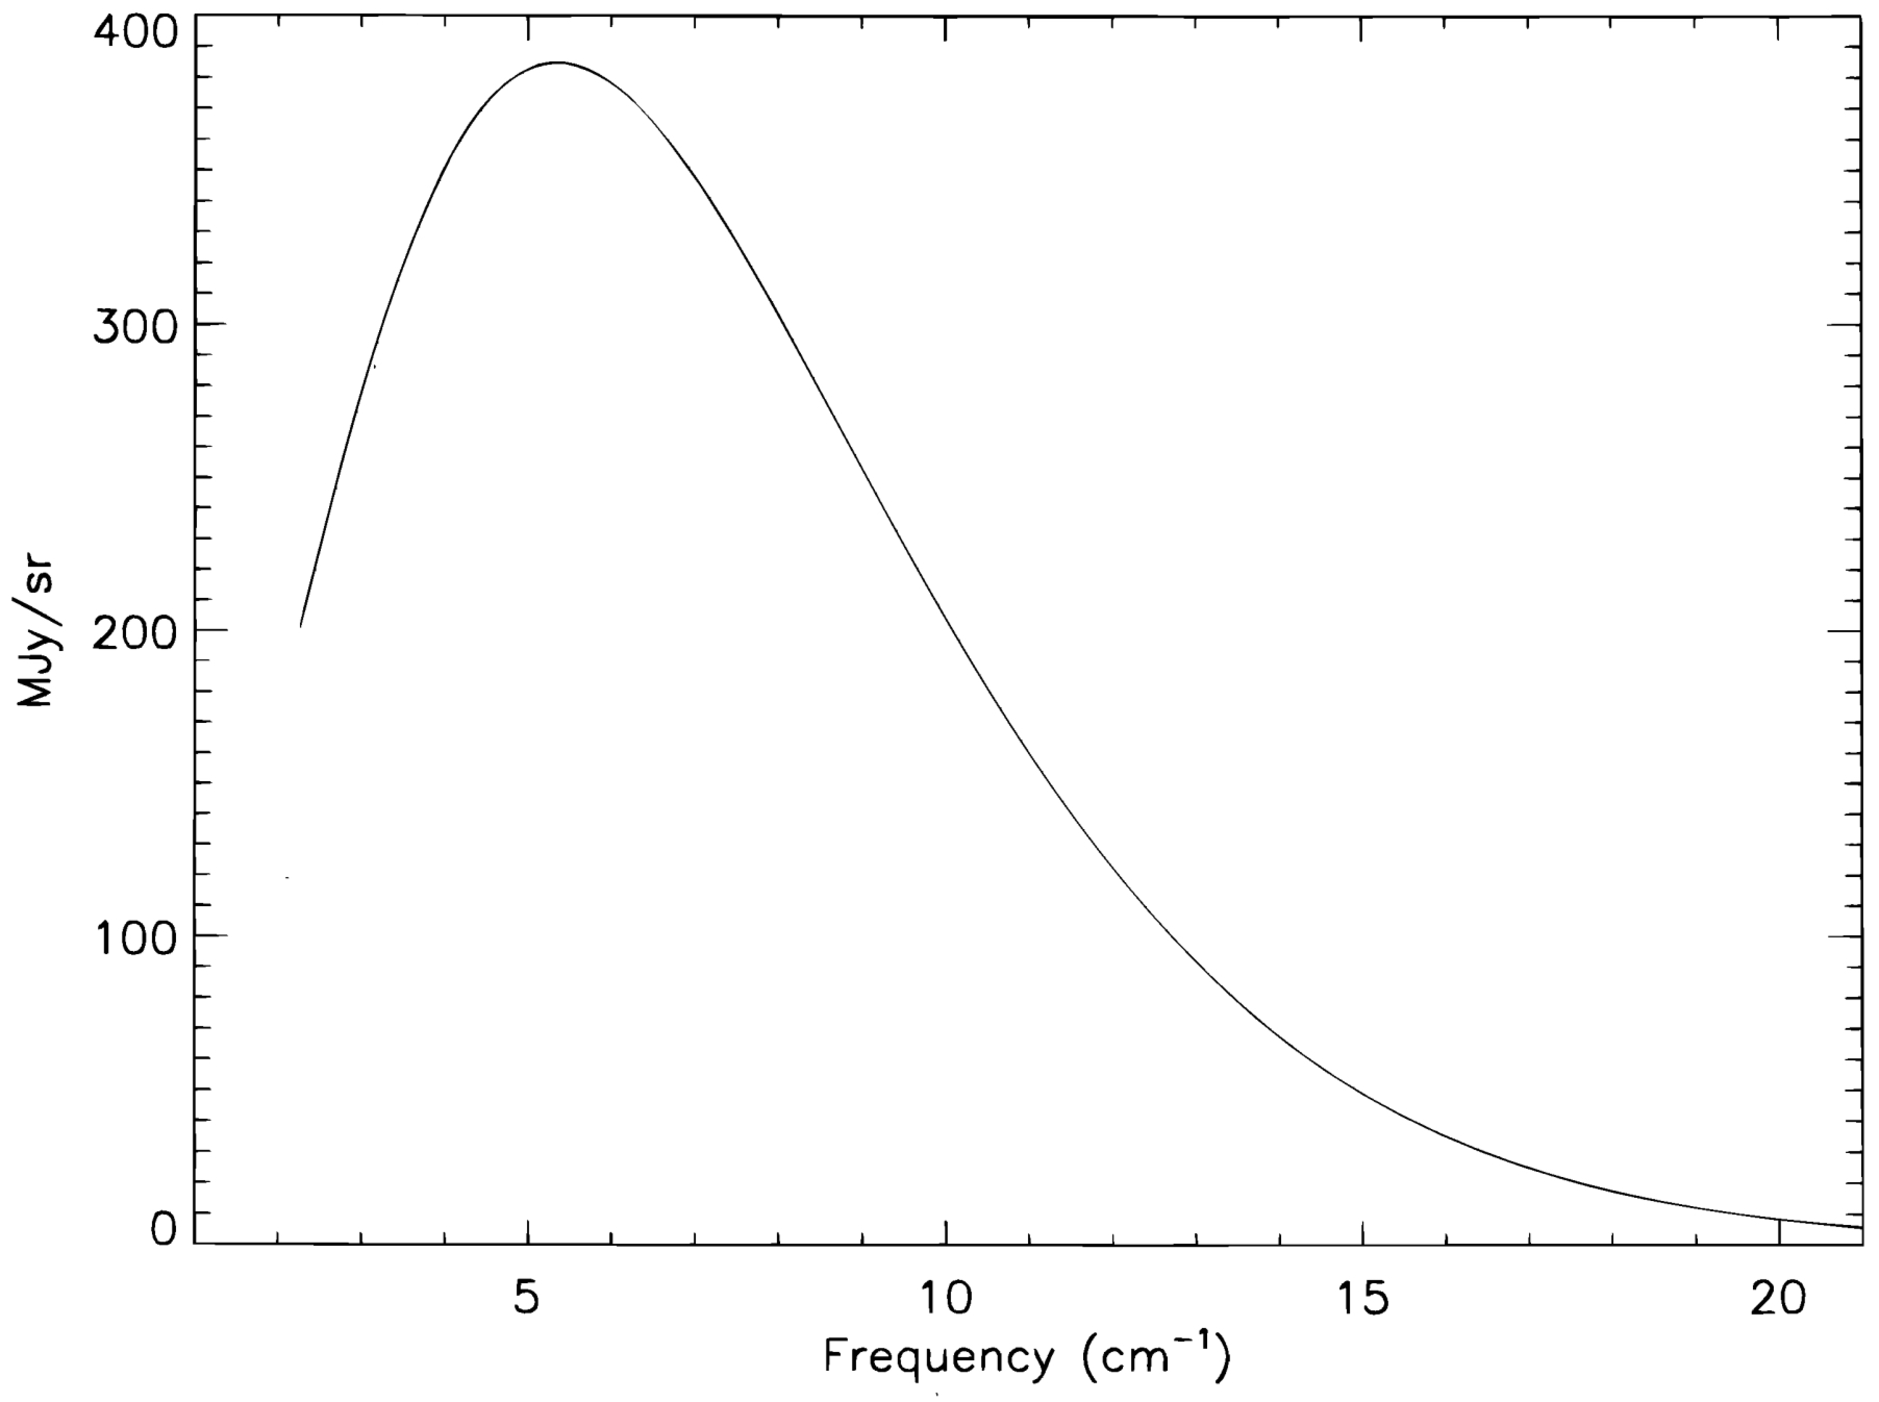
\includegraphics[width=0.6\textwidth]{cobe.pdf}
    \caption{COBE衛星によるCMBのスペクトル測定結果。}
    \label{fig:cobe}
\end{figure}

\section{$\Lambda\mathrm{CDM}$モデル}

\section{インフレーション宇宙論}

\section{CMB偏光モード}
\section{本論文の構成}

\end{document}